%% APJ Doc Class
%\documentclass[preprint,12pt]{aastex} % one-column
%\documentclass[preprint2]{aastex} % two-column
\documentclass[apjl]{emulateapj}

%% Packages
\usepackage{xspace}
\usepackage{color}
\usepackage{rotating}
%\usepackage{multicol}
\usepackage{amsmath}
\usepackage{subfigure}
%\PassOptionsToPackage{hyphens}{url}\usepackage{hyperref}

%% Custom commands for figs/edits
\newcommand{\xxx}[1]{{\color{red} #1}} % \xxx makes things RED
\def\imagebox#1#2{\vtop to #1{\null\hbox{#2}\vfill}} % http://tex.stackexchange.com/questions/152818/top-aligned-subfigure-with-bottom-aligned-caption

%% ApJ style
\bibliographystyle{apj}

%% Slugcomment
\slugcomment{Draft version \today}

%% Short title, authors
\shorttitle{Exo-Aurorae on Proxima Centauri \MakeLowercase{b}}
\shortauthors{Luger et al.}

%% Begin Doc
\begin{document}

%% Title, authors, affils
\title{The Pale Green Dot: A Method to Characterize Proxima Centauri \MakeLowercase{b} using Exo-Aurorae}

\author{Rodrigo Luger\altaffilmark{1,3,4,6}}
\author{Jacob Lustig-Yaeger\altaffilmark{1,3,4}}
\author{David P. Fleming\altaffilmark{1,3,5}}
\author{Matt A. Tilley\altaffilmark{2,3,4}}
\author{Eric Agol\altaffilmark{1,3,4}}
\author{Victoria S. Meadows\altaffilmark{1,3,4}}
\author{Russell Deitrick\altaffilmark{1,3,4}}
\author{Rory Barnes\altaffilmark{1,3,4}}



\altaffiltext{1}{Astronomy Department, University of Washington, Box 951580, Seattle, WA 98195}
\altaffiltext{2}{Department of Earth \& Space Sciences, University of Washington, Box 351310, Seattle, WA 98195}
\altaffiltext{3}{NASA Astrobiology Institute -- Virtual Planetary Laboratory Lead Team, USA}
\altaffiltext{4}{Astrobiology Program, University of Washington, 3910 15th Ave. NE, Box 351580, Seattle, WA 98195, USA}
\altaffiltext{5}{eScience Institute, University of Washington, Seattle, WA, USA}
\altaffiltext{6}{\email{rodluger@uw.edu}}

%% Abstract %%

\begin{abstract}
We examine the feasibility of detecting auroral emission from the potentially habitable exoplanet Proxima Centauri b. This planet's active, late-type M dwarf host makes detection of aurorae more favorable, primarily by increasing auroral power and improving the planet-star contrast in the visible wavelength range due to strong TiO absorption in the star. Detection of aurorae would yield an independent confirmation of the planet's existence, constrain the presence and composition of its atmosphere, and determine the planet's eccentricity and inclination, thereby breaking the mass-inclination degeneracy. We use two independent methods to estimate that the auroral power on Proxima b is ${\sim} 100 {\times}$ stronger than that on Earth under steady-state stellar wind if Proxima b is a terrestrial world with an atmosphere and magnetic field. These estimates indicate a planet-star contrast ratio of $\gtrsim 10^{-6}$ in a narrow band about the green 5577\AA\ OI auroral emission line, although higher contrast may be possible during periods of magnetospheric disturbance. We find that detection of 10 terawatt aurorae may be possible with 10 meter class facilities in ${\sim} 1$ day of exposure time with a signal-to-noise ratio of 6 if used in combination with visible-light adaptive optics and coronagraphic starlight suppression. We searched the high spectral resolution Proxima b HARPS data for the 5577\AA\ line and for other prominent oxygen and nitrogen lines, but find no signal, indicating that oxygen green line auroral emission on Proxima Centauri must be below ${\sim} 10^{15}$ W (${\sim} 3\times 10^4$ times stronger than on Earth), consistent with our predictions.  Future detection with a large-aperture, space-based coronagraphic telescope or a ground-based extremely large telescope with coronagraph could push sensitivity down to terawatt oxygen aurorae with exposure times of ${\sim} 100$ hours at high spectral resolution. 
\end{abstract}

%% Keywords %%
\keywords{planets and satellites: terrestrial planets, atmospheres, aurorae, detection --- \object{Proxima Centauri b}}

%% Introduction %%

\section{Introduction\label{sec:intro}}

The discovery of Proxima Centauri b (henceforth `Proxima b'), at only 1.3pc from the Sun, ushers in a new era of potentially habitable exoplanet science because of the rich characterization potential afforded by its proximity \citep{Anglada-Escude2016}.  Although Proxima b is not known to transit---making transmission spectroscopy impossible---it is an ideal candidate for high-contrast direct spectroscopy using an extremely large coronagraph-equipped telescope. However, even with the enhancement in angular resolution provided by the proximity of its host star, Proxima b's close-in orbit \citep[$a = 0.0485$ AU;][]{Anglada-Escude2016} precludes imaging with current coronagraphs, such as the Gemini Planet Imager \citep[GPI;][]{Macintosh2014} and the Very Large Telescope's Spectro-Polarimetric High-contrast Exoplanet REsearch \citep[VLT-SPHERE;][]{Beuzit2008}, which operate primarily in the near-infrared. This is in part due to the poorer Strehl ratios currently achievable at visible wavelengths with ground-based adaptive optics (AO) systems\footnote{See, e.g., \url{https://www.eso.org/sci/facilities/paranal/instruments/sphere/overview.html}}. Consequently, in advance of larger diameter ground- and space-based telescopes, and improvements in visible AO systems, we must initially consider observations that do not rely on transits or current coronagraphy to search for and characterize the atmosphere of Proxima b.

Phase curves may offer one of the first means to study the atmosphere of Proxima b \citep{Turbet2016,Kreidberg2016,Meadows2016} by potentially showing the reduction in day-night thermal emission contrast associated with an atmosphere. Phase curves have proven to be a successful means to characterize the atmospheres of planets larger and hotter than Proxima b \citep{Cowan2007, Knutson2007, Knutson2008, Crossfield2010, Brogi2012, Zellem2014, Stevenson2014}, including ones that do not transit \citep{Selsis2011, Faigler2011, Maurin2012, Brogi2014}. However, the expected planet-to-star contrast ratio in the visible and NIR due to reflected stellar radiation is likely to be below the anticipated systematic noise floor for JWST/NIRSpec \citep{Meadows2016}, and although the planet-star contrast ratio becomes quite favorable beyond 10 $\mu$m, where the planetary thermal emission peaks, mid-IR phase curves will require JWST/MIRI. Given the uncertainty of the expected phase-curve studies with JWST, it is worthwhile to investigate novel methods for characterizing the atmospheric state of Proxima b. 

To complement the anticipated JWST thermal phase curve measurements, in this work we explore the possibility of directly detecting optical auroral emission from the atmosphere of Proxima b using high-resolution optical spectroscopy. Numerous studies have investigated exoplanet aurorae in the radio due to cyclotron and synchrotron emission to constrain the planetary magnetic field \citep[e.g.][]{Bastian2000,Grie2007,Zarka2007,Hess2011,Driscoll2011}. \citet{Smith2004} modeled the role of aurorae in redistributing high energy incident stellar flux to the surface of terrestrial exoplanets, and the effect of aurorae on the optical and infrared spectra of gaseous exoplanets has been considered \citep{Rimmer2015}. However, the detection of auroral emission from the atmosphere of nearby terrestrial exoplanets and the physical constraints imposed by such a detection have not been fully discussed. 

Detecting optical auroral emission from the possible atmosphere of Proxima b is likely much more favorable for this system than for an Earth-Sun analog. This is due to both planetary and stellar characteristics that favor auroral production and improve detectability. In particular, Proxima b's intrinsic planetary properties may favor production of aurorae from O atoms. If Proxima b is Earth-like in composition, recent dynamical/planetary interior modeling results by \citet{Barnes2016} and \citet{Zuluaga2016} suggest that the planet is likely to have a magnetic field, potentially increasing the likelihood of atmospheric retention and of auroral emission. Atmospheres rich in oxygen-bearing molecules, including O$_2$ and CO$_2$, have been predicted for Proxima b \citep{Meadows2016} as a result of the evolutionary processes for terrestrial planets orbiting M dwarfs \citep{LugerBarnes2015,Barnes2016}. On Earth, the oxygen auroral line at 5577\AA\ provides the distinctive green glow observed in both the Aurora Borealis\footnote{Also known as the Northern Lights, which enables nighttime-viewing of queer sights \citep{Service1907}.} and the Aurora Australis, and is the brightest auroral feature \citep{Chamberlain1961, Dempsey2005}. For emissions from the upper atmosphere, only the 1.27$\mathrm{\mu}$m O$_2$ airglow and combined near-infrared OH nightglow features are brighter \citep{Hunten1967}. The oxygen green line is seen in both the Earth's O$_2$-rich atmosphere \citep{Chamberlain1961} and Venus' CO$_2$-dominated atmosphere \citep{Slanger2001}, where it has been observed to increase in brightness after CME events \citep{Gray2014}.

The stellar properties and the planet-star separation are also likely to enhance the auroral power on Proxima b relative to an Earth-Sun analog. Proxima Centauri is an active flare star with a magnetic field ${\sim} 600\times$ stronger than that of the Sun \citep{Reiners2008,Davenport2016}. Since stellar activity drives auroral emission, such features may be much stronger on planets orbiting active M dwarfs. Additionally, with a close-in orbit of 0.0485 AU, Proxima b is about $20\times$ closer to Proxima Centauri than the Earth is to the Sun \citep{Anglada-Escude2016}. This proximity further increases particle fluxes incident on the planetary atmosphere that drive ionization and the subsequent recombination radiation.

In addition to increasing the likelihood and strength of the aurora, the characteristics of the Proxima Centauri system may also enhance its detectability. Since the Proxima system is only 1.3pc away, it is perhaps the best-case scenario for the detection of the faint auroral signal from a terrestrial exoplanet. Even though the planet-star contrast ratio in reflected visible light is poor \citep[${\sim} 10^{-7}$; see][]{Turbet2016,Kreidberg2016,Meadows2016}, if Proxima b exhibits auroral emission, this will brighten the planet and boost the planet-star contrast by a few orders of magnitude at the wavelengths of the auroral emission features. The short wavelength of the oxygen green line also improves the contrast of the planet relative to the star due to the star's cool temperature and TiO absorption, which strongly suppresses the brightness of the star in the visible. This improvement in contrast is significantly less for the near-infrared O$_2$ 1.27$\mathrm{\mu}$m and OH airglow lines. In addition to increasing the contrast, the small semi-major axis of Proxima b results in an orbital velocity of ${\sim} 50$ km/s, which will cause its auroral emission to be Doppler-shifted by as much as 1\AA\ over the course of its orbit, making it easier to disentangle it from stellar features via high resolution spectroscopy. An additional advantage of the short wavelength is the smaller inner working angle and point-spread function that may be achieved with a coronagraph at shorter wavelength \citep{Agol2007}. These factors all improve the chance of detection with ground-based telescopes.

The detection of the oxygen auroral line at 5577\AA\ would provide an important diagnostic for planetary properties. Its detection would not only confirm the presence of the planet, but would point to the presence of an atmosphere with abundant oxygen atoms, which is more likely to indicate a terrestrial body. Additionally, the detection of the line would yield a measurement of the radial velocity (RV) of the planet, which combined with the RV measurements of the star \citep{Anglada-Escude2016} would enable the measurement of the eccentricity and inclination of the orbit, ultimately yielding the mass of the planet. Detection of the oxygen auroral line would therefore provide several key planetary parameters that could be used to constrain Proxima b's potential habitability \citep{Barnes2016,Meadows2016}.

%[Pre-Vikki text] Detecting optical auroral emission from the possible atmosphere of Proxima b is likely more favorable for this system than for an Earth-Sun analog. First, Proxima Centauri is an active flare star with a magnetic field $\sim 600 \times$ stronger than that of the Sun \citep{Reiners2008,Davenport2016}. Since stellar activity drives auroral emission, such features may be much stronger on planets orbiting active M-dwarfs. Second, the semi-major axis (0.0485 AU) places Proxima b about $20 \times$ closer to Proxima Centauri than the Earth-Sun distance \citep{Anglada-Escude2016}. This proximity further increases particle fluxes incident on the planetary atmosphere that drive ionization and the subsequent recombination radiation. As the planet is deeper in the gravitational well of its star than Earth is in the Sun's, its orbital velocity $\sim 50$ km/s is larger than the Earth's, $\sim 30$ km/s,  its auroral emission will be Doppler-shifted by about 1\AA\ over the course of its orbit, making it easier to disentangle it from stellar features. Third, although the planet-star contrast ratio in reflected visible light is poor  \citep[${\sim} 10^{-7}$; see][]{Turbet2016,Kreidberg2016,Meadows2016}, if the planet exhibits auroral emission, this added source term can boost the planet-star contrast several orders of magnitude in the small wavelength range within each auroral emission feature. Fourth, atmospheres rich in oxygen-bearing molecules have been predicted for Proxima b \citep{Meadows2016}. On Earth, the oxygen auroral line at 5577\AA\ provides the distinctive green glow observed in both the Aurora Borealis\footnote{Also known as the Northern Lights, which enables nighttime-viewing of queer sights \citep{Service1907}.} and the Aurora Australis and dominates the aurora flux budget \citep{Chamberlain1961,Dempsey2005}. This line has been well studied on both Earth \citep{Chamberlain1961} and Venus \citep{Crisp1996,Slanger2001}. Fifth, Proxima b resides only 1.3 pc away and is perhaps the best-case scenario for the detection of a faint auroral signal from the atmosphere of a terrestrial exoplanet.  Sixth, recent results by \citet{Barnes2016} and \citet{Zuluaga2016} suggest that if Proxima b is Earth-like in composition, it likely has a magnetic field, increasing the likelihood of atmospheric retention and hence auroral emission. Seventh, the short wavelength of the oxygen line improves the contrast of the planet relative to the star due to the star's cool temperature and TiO absorption band. An additional advantage of the short wavelength is the smaller inner working angle and point-spread function that may be achieved with a coronagraph at shorter wavelength \citep{Agol2007}. These factors improve the chance of detection with ground-based telescopes. Eighth, the detection of the line would enable the measurement of the inclination of the orbit, yielding the mass of the planet. Finally, a detection of the oxygen auroral line at 5577\AA\ would not only confirm the presence of the planet, but would also confirm the presence of an atmosphere with oxygen-bearing species, which can be used to constrain its potential habitability \citep{Barnes2016,Meadows2016}.

This paper is organized as follows: in \S\ref{sec:signal} we calculate the expected total auroral emission strength of Proxima b. In \S\ref{sec:detect} we model the planet-star contrast ratio assuming oxygen auroral emission and calculate the integration time required to detect the feature. In \S\ref{sec:search} we conduct a preliminary search for auroral emission in the HARPS high-resolution, ground-based spectroscopy used by \citet{Anglada-Escude2016} for the RV detection of Proxima b. Finally, in \S\ref{sec:disc} we discuss our results and present our conclusions.

%%%%%%%%%%% Extra intro notes to maybe include %%%%%%%%%%%%%
% - Lots of previous research on Earth's magnetosphere, aurora, solar winds, i.e. entire field of space physics.
%
% - Detections of aurora on Venus
%
% - Lots of interest in M dwarf habitability and impact of stellar magnetic field and solar winds on close-in planets
%
% - It may be possible to discriminate between an auroral feature due to a terrestrial planet versus a Jovian planet (Driscoll et al., 201..). Moreover, such a discrimination may help constrain the inclination of the planet since the mass of a Jovian planet will only be consistent low inclination solutions.
%%%%%%%%%%%%%%%%%%%%%%%%

%% Section: Signal Estimation %%

\section{Auroral Signal Strength}
\label{sec:signal}

 %% Matt's edits below, feel free to move
%It has been suggested that the stellar activity of Proxima Centauri and close orbit of Proxima b could result in auroral intensities up to 10$^3\times$ stronger than Earth's \citep{OMalley2016}. 
Below, we quantitatively estimate the auroral intensity for steady-state stellar input. We employ two different methods to compare and contrast the regimes for both an Earth-like and a Neptune-like planetary magnetic dipole moment and anticipated auroral production efficiency. Both planets are assumed to be terrestrial bodies with the orbital characteristics of Proxima b. Method 1 involves a simple estimation of the auroral brightness driven by the stellar wind power delivered at the magnetopause of the planet. Method 2 uses the prediction of a magnetohydrodynamical (MHD) model that was empirically tuned to calculate the auroral response at Earth, with modifications to the relevant inputs of the stellar wind of Proxima Centauri and assumed planetary parameters for Proxima b \citep{Anglada-Escude2016}. 

The quantities we calculate include only the localized emissions caused by magnetospheric particle precipitation into a discrete auroral oval, not the diffuse, global phenomenon of airglow. On Earth, the 5577\AA\ airglow can be visible to the naked eye and could be significant on Proxima b, but is driven by different physical processes (e.g., nighttime recombination due to dayside photoionization) that are out of scope for this analysis. Similarly, the 5577\AA\ airglow has been observed at Venus \citep[e.g.][]{Slanger2001} and Mars \citep[e.g.][]{Seth2002} --- both of which have no global magnetic field. For these reasons we cannot suggest basing the existence of or placing constraints on Proxima b's planetary magnetic field based on the detection of this auroral line.

%Method three follows a brightness model treatment of the auroral response of Ganymede in the Jovian magnetosphere. 
%The methods below are representative of the steady-state stellar wind, and do not take into account transient increases due to stellar magnetic activity.

\subsection{Auroral stellar wind power scaling}
\label{sec:signal_m1}

%% Fig: Method 1 - stellar wind scaling %%
\begin{figure}[bt]
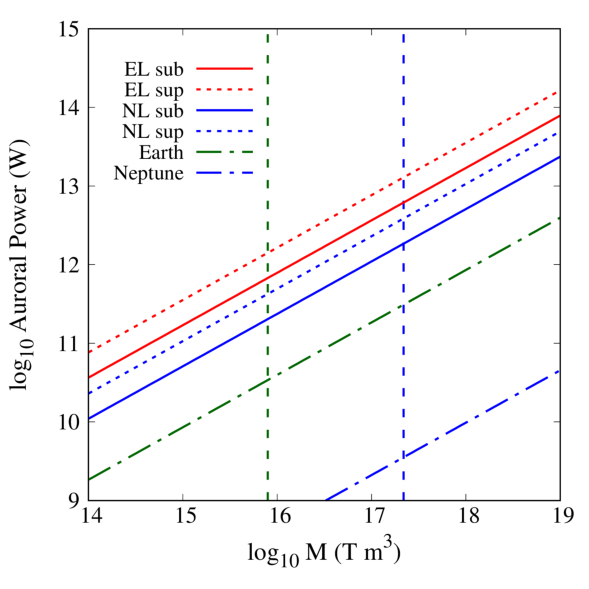
\includegraphics[width=0.47\textwidth, angle=0]{plot_swpower.pdf}
\caption{Estimated auroral power as a function of planetary magnetic dipole moment calculated using the stellar wind scaling method from \S\ref{sec:signal_m1}. Solid (dotted) lines correspond to the sub-(super-)Alfv\'{e}nic stellar wind conditions. Red (blue) lines correspond to an Earth-like (Neptune-like) planetary magnetic dipole with conversion efficiency of $\sim$1\% ($\sim$0.3\%). The green (blue) dash-dotted lines correspond to Earth (Neptune) in its natural orbit around the Sun. The dashed vertical green (blue) line indicates the magnitude of Earth's (Neptune's) magnetic dipole moment.\\[0.01in]}
\label{fig:auroral_power}
\end{figure}
%%%%%%%%%%%%%%%%%%%

M dwarf mass-loss rates, and therefore stellar winds, are not well constrained due to observational sparsity and difficulty \citep[e.g.][]{Wood2004}. To model the M dwarf winds for Proxima Centauri, we adopt the predictions from the modeling efforts of \citet{Cohen2014}, who generated an MHD stellar wind model for the M3.5 star EV Lacertae based on available observations. \citet{Wood2005} estimated that the mass-loss per unit surface area for Proxima Centauri and EV Lacertae as quite similar, which sets the wind conditions at distances in stellar radii to be comparable. Here, we consider both super- and sub-Alfv\'{e}nic conditions for the steady-state stellar wind, using the reported parameters at Planet C (simulated for $a\approx 90 R_\star$, similar to Proxima b) from \citet{Cohen2014}; see Table~\ref{tab:swparams}.
 
\begin{deluxetable}{ccccc}

\tablewidth{\linewidth}
\tablecaption{Stellar wind conditions}
\tablenum{1}
\tablehead{\colhead{Quantity} & \colhead{Sub-Alfv\'{e}nic} & \colhead{Super-Alfv\'{e}nic} } 
\startdata
n (cm$^{-3}$) & 46 & 123  \\
T (10$^5$ K) & 4.98 & 1.9 \\
{\bf u} (km $s^{-1}$) & (-728, -50, -17) & (-660, 8, 14) \\
{\bf B} (nT) & (240, 88, 17) & (-244, 74, 18) \\
M$_{A}$ & 0.88 & 1.3
\enddata
\tablecomments{Stellar wind conditions from \citet{Cohen2014}. \label{tab:swparams}}

\end{deluxetable}

The stellar wind power delivered to the magnetosphere of the planet can be expressed as

\begin{align}
    P_{SW} = \rho v^3 \pi R_{MP}^2, \label{eq:swpower}
\end{align}

\noindent where $\rho$ and $v$ are the stellar wind mass density and velocity, respectively, and $R_{MP}$ is the magnetopause distance along the line connecting the star and planet (sub-stellar point). The latter can be estimated through magnetospheric pressure balance with the total stellar wind pressure:
\begin{align}
    \frac{\mathcal{M}^2}{2 \mu_0 R_{MP}^6} = p_{KE} + p_{ram} + p_{B}, \label{eq:pressbal}
\end{align}
%\noindent The term on the LHS is the magnetospheric magnetic pressure, given by the dipole magnetic field of the planet, $B_P=\mathcal{M}/R_P^3$, 
where $\mathcal{M}$ represents the magnitude of the magnetic dipole moment and $R_{MP}$ is the distance from the planet at which the magnetic pressure of the planet balances the pressure of the stellar wind. The terms on the RHS of Eq.~\ref{eq:pressbal} represent the kinetic ($p_{KE}=n k_B T$), dynamic ram ($p_{ram}=\rho v^2$), and magnetic ($p_B=B_{SW}/2 \mu_0$) pressures of the stellar wind, calculated from the values in Table~\ref{tab:swparams}. 
%Solving Eq.~\ref{eq:pressbal} for R$_P$ gives us the magnetopause balance point, R$_{MP}$:
%\begin{align}
%    R_{MP} = \left(  \frac{\mathcal{M}^2}{2 \mu_0 (p_{KE} + p_{ram} + p_{B})} \right)^{1/6}. \label{eq:rmp}
%\end{align}
For the Earth-like, EL, (Neptune-like, NL) magnetosphere, we assume a magnetic dipole moment of $\mathcal{M}=8.0\times$10$^{15}$ (2.2$\times$10$^{17}$) Tesla m$^3$. Solving for $R_{MP}$ in Eq.~\ref{eq:pressbal} and inserting into Eq.~\ref{eq:swpower} provides an estimate of the stellar wind power incident on the planetary magnetopause. Externally-driven planetary auroral systems are not typically 100\% efficient at converting the incident stellar wind power into auroral emission, and range from $\sim$0.3\% at Neptune, $\sim$1\% at Earth, and up to $\sim$100\% at Jupiter \citep[e.g.][]{Cheng1990,Bhardwaj2000}. For reference, at Earth, this method gives us a reasonable estimate of the total auroral power of $\sim$30 GW for nominal solar wind conditions (5 cm$^{-3}$, 400 km s$^{-1}$, 10 eV protons), which is consistent with the anticipated power of 1-100 GW, depending on solar and magnetospheric activity.

Fig.~\ref{fig:auroral_power} shows the predicted auroral power from Eq.~\ref{eq:swpower} for both EL and NL planetary magnetic dipole moments and conversion efficiencies in both the sub- and super-Alfv\'{e}nic stellar wind conditions from Table~\ref{tab:swparams}. Auroral power estimates for both the EL and NL planets at 0.05 AU are shown in Table~\ref{tab:auroral_power}. The total emitted power ranges from $\sim$22.3$\times$ Earth's auroral emission (EL, sub-Alfv\'{e}nic) to $\sim$130$\times$ (NL, super-Alfv\'{e}nic). Note that discussion of a true, $\sim$17.15 Neptune-mass planet is included below in \S~\ref{sec:signal_m2}.
%A factor of 10$^3$ increase is likely to be a transient state for auroral emission, driven only by strong magnetospheric substorm onset. However, given the high activity of Proxima Centauri as reported by \citet{Davenport2016}, it could be a more common state - even a consistent one - for Proxima b compared to Earth. Detailed global magnetospheric modeling is needed to determine the substorm frequency in response to such strong stellar activity. % Discussion point

Note that Neptune's magnetic field is highly inclined, rotationally offset, and relatively complex with significant quadrupole/octupole moments that have similar or higher magnitude than the dipole moment; in the present work, we have assumed a simple, untilted dipole field, with equatorial strength equal to that reported by Voyager 1 observations \citep[e.g.][]{Connerney1991,Mauk2012}. The auroral power estimate for Neptune in Fig.~\ref{fig:auroral_power} ($\sim$3 GW) makes these same geometric assumptions, leading to an overestimate when compared to the actual auroral power emitted at Neptune.

We scale the total auroral power values in Table~\ref{tab:auroral_power} by 60\% (assuming lower energy particle populations present in a quiescent magnetosphere) to obtain estimated emission power of the OI 5577\AA\ line \citep{Chamberlain1961,Kivelson1995}. From this method, we predict an emitted power of $\sim$0.41 (1.12) TW for the EL (NL) planet in the sub-Alfv\'{e}nic stellar wind, and $\sim$0.852 (2.33) TW for the super-Alfv\'{e}nic conditions for the 5577\AA\ line.

\begin{deluxetable}{lccc}

\tablewidth{\linewidth}
\tablecaption{Calculated emitted total auroral power, by method}
\tablenum{2}
\tablehead{\colhead{Case} & \colhead{Method 1} & \colhead{Method 2} \\
\colhead{} & \colhead{[TW]} & \colhead{[TW]}} 
\startdata
EL$_{\text{Sub}}$ & 0.68 & 1.09  \\
NL$_{\text{Sub}}$ & 1.86 & 10.00 \\ 
EL$_{\text{Sup}}$ & 1.42 & 1.09  \\
NL$_{\text{Sup}}$ & 3.88 & 10.00
\enddata
\tablecomments{Total emitted power for the Earth-like (EL) and Neptune-like (NL) planets in the sub-Alfv\'{e}nic (Sub) and super-Alfv\'{e}nic (Sup) stellar wind. \label{tab:auroral_power}}

\end{deluxetable}

\subsection{3D MHD empirical energy coupling}
\label{sec:signal_m2}
 
\citet{Wang2014} developed a global, 3D MHD model to obtain a nonlinear fit to the energy coupling function to estimate the energy transferred from the solar wind to Earth's auroral activity (see their Eq.~13). %The resulting fit for the energy transfer to the terrestrial magnetosphere was found as:
 %
%\begin{align}
%    P = K_1\,n_{sw}^{0.24}\,v_{sw}^{1.47}\,B_T^{0.86}\,\left[\sin^{2.7}(\theta/2)+0.25 \right] \label{eq:mhd_fit},
%\end{align}
% 
%\noindent where K$_1=$3.78$\times$10$^7$ is a coupling constant, $n_{sw}$ and $v_{sw}$ are the stellar wind number density (in cm$^{-3}$) and velocity (in km s$^{-1}$), respectively, $B_T$ is the magnitude of the transverse component of the Sun's interplanetary magnetic field (IMF) ($B_T = \sqrt{B_X^2+B_Y^2}$) in nT, and $\theta$ is the so-called IMF clock angle ($\tan(\theta) = B_Y/B_Z $). The coordinate system used is the geocentric solar magnetospheric (GSM) system, with $\hat{X}$ pointing from the planet to the star, $\hat{Z}$ aligned with the magnetic dipole axis of the planet (here assumed to be perpendicular to the ecliptic), and $\hat{Y}$ completing a right-handed coordinate system. 
As this system takes into account only the Earth's magnetosphere, we require it to scale to other planetary magnetic fields -- such as Neptune's -- by noting the coupling scales with the planetary magnetic dipole magnitude, $\mathcal{M}_P^{2/3}$ \citep{Vasyliunas1982}. Therefore, $(\mathcal{M}_{Nep}/\mathcal{M}_{Earth})^{2/3}\approx \, 9.1$, which we can fold into the coupling constant for an NL planet.%, i.e. $K_1\sim$3.44$\times$10$^8$.
 
\citet{Wang2014} estimate the fraction of total solar wind energy input to the entire magnetosphere is $\sim$13\% of the incident energy. They further estimate that 12\% of that energy is dissipated by particle precipitation in the auroral regions, yielding a total solar wind/auroral coupling efficiency of $\sim$1.56\% -- very similar to the value assumed in \S~\ref{sec:signal_m1} for the EL planet. This method predicts a maximum coupling of auroral particle precipitation (with interplanetary magnetic field clock angle $\theta =$ $\pi$, driving reconnection and likely substorm activity) at Earth (Neptune) of $\sim$222.6 (2.8) GW, which is in order of magnitude agreement with terrestrial plasma observations \citep[e.g.][]{Hubert2002} and inferred values from Voyager UV measurements \citep[e.g.][]{Sandel1990,Mauk1994}. 

For Proxima b, this method predicts a total power of auroral particle precipitation of 11.82 (107.55) TW for the EL (NL) planet in the sub-Alfv\'{e}nic stellar wind, and 12.39 (112.78) TW in the super-Alfv\'{e}nic wind. To compare directly to the total auroral power output such as that calculated in \S~\ref{sec:signal_m1}, we must link these values to the aurora by including the efficiency of precipitating charged particles in the production of auroral emission for the 5577\AA\ line, as below.

\citet{Steele1990} reported coordinated ground-based observations of auroral line intensities and the related satellite observations of energetic electron flux to draw a relation between electron precipitation and auroral brightness. For the 5577\AA\ OI line, 1.73$\pm$0.51 (1.23$\pm$0.44) kR/(erg cm$^{-2}$ s$^{-1}$) was observed for a Maxwellian electron population of characteristic temperature 1.8 (3.1) keV, which corresponds to an efficiency of 0.62\% (0.44\%) in conversion of incident flux to OI flux (1 R $\equiv 10^{6}/4\pi\ \mathrm{s^{-1}\ cm^{-2}\ sr^{-1}}$). It is worth noting that the fraction of total hemispheric particle energy delivered by electrons is $\sim$80\%, varying by 10-20\% due to magnetospheric activity \citep{Hubert2002}.

The magnetopause distance we calculated via Eq.~\ref{eq:pressbal} for the EL (NL) magnetic dipole moment, $\sim$5.7 (17.2) $R_P$, can provide a simple estimate of the total auroral oval coverage. The magnetic co-latitude of the boundary between open and closed flux is sin$^{-1}$(1/$\sqrt{R_{MP}}$); if we assume a nominal 5$^\circ$ auroral oval width centered at the co-latitude obtained, we calculate a single-hemisphere coverage of $\sim$9.2$\times$10$^{16}$ (5.2$\times$10$^{16}$) cm$^2$ for the auroral oval of the EL (NL) planet.
 
 Using the average of the efficiencies given by \citet{Steele1990} above, we obtain a brightness value of 1.59 (25.8) MR for the EL (NL) planet for the 5577\AA\ line for the sub- and super-Alfv\'{e}nic conditions. This corresponds to an emission power of $\sim$0.65 (6) TW for the 5577\AA\ line per hemisphere. Assuming that 60\% of auroral power is emitted as the 5577\AA\ line under nominal, non-substorm conditions, we obtain a total auroral power of 1.1 (10) TW. These values are comparable to those obtained in \S~\ref{sec:signal_m1}, and more favorable for the stronger NL dipole, as expected. Note that the values are similar for the sub- and super-Alfv\'{e}nic cases, as the method from \citet{Wang2014} is weighted more heavily towards the velocity and IMF clock angle of the stellar wind; as seen in Table~\ref{tab:swparams}, the wind parameters are comparable in most regards, including the velocity and clock angle, and therefore give matching results within 5\%.

%If Proxima b is instead a true Neptune-like planet (not just magnetic dipole strength), it will likely exhibit an H/H$_2$ upper atmosphere. 
If Proxima b is, instead, a planet of Neptune mass and radius (as opposed to our assumption of only the magnetic parameters) on a close to face-on orbit, it will have an upper atmosphere dominated by H/H$_2$. Therefore the above calculations are not applicable, and we should consider FUV emission in lieu of OI or N$_2^+$ lines. Voyager UV observations reported by \citet{Sandel1990} estimated the localized FUV (967-1115 \AA) auroral brightness as $\sim$5 R. \citet{Mauk1994} found that the electron flux to drive the observed UV aurora at Neptune was $\sim$10$^{-3}$ erg cm$^{-2}$ s$^{-2}$. Therefore we infer a conversion efficiency for Neptune's aurora in the 967-1115 \AA\ bandpass to be $\sim$5 kR/(erg cm$^{-2}$ s$^{-1}$), corresponding to~$\sim$9.9\%. This gives us a scaled FUV brightness of $\sim$4.02 (4.22) MR for the sub-(super-)Alfv\'{e}nic stellar wind conditions for the Neptune-like planet, or 19.43 (20.39) TW over the 967-1115 \AA\ band. While this is significantly stronger than the OI emission of an Earth-like planet, it may be harder to detect given both the width of this band and the fact that if Proxima b is Neptune-like, its orbital inclination must be $\lesssim 5^\circ$, making deconvolution from stellar lines more difficult (see \S\ref{sec:search}).

It is possible that all the auroral numbers reported for the sub-Alfv\'{e}nic cases above could be a factor of 4-5 (or more) larger. We are assuming a simple dipolar, Earth-Sun like interaction with the sub-Alfvenic stellar wind, which isn't specifically the case for sub-Alfvenic flow; these interactions are more akin to the interactions of Ganymede and Io with the corotating magnetosphere of Jupiter, with the formation of Alfven wings. Modeling efforts by \citet{Preusse2007} showed that for a giant planet with a dipole magnetic moment, field-aligned currents (which are associated with auroral activity) are significantly stronger for planets orbiting inside the Alfv\'{e}n radius of their stellar host. Our estimates, therefore, could be viewed as lower limits. It is also worth noting that \citet{Cohen2014} suggested that a transition between the sub- and super-Alfv\'{e}nic conditions would likely produce enhanced magnetospheric activity and therefore could lead to a periodicity in the auroral activity depending on combined planetary orbital and stellar rotational phases. For Earth, the diffuse airglow at 5577 \AA\ can be significant ($\geq$ 1 kR), but the anticipated magnitude at Proxima b is unknown, and could be another factor that contributes to the overall signal. Detailed photochemical modeling is required to obtain an estimate of airglow production.

In summary, we predict an auroral emission at 5577\AA\ that is of order 10-100 times stronger than seen on Earth for steady-state stellar wind conditions and a quiet magnetosphere, corresponding to a total auroral power on the order of ${\sim} 1$ TW for an Earth-like terrestrial planet orbiting Proxima Centauri. The predicted values will naturally change based on planetary parameters (e.g., magnetic dipole moment, magnetospheric particle energy distributions, substorm onset, atmospheric Joule heating) and stellar activity. By our analysis, the ${\sim} 10^3$ enhancement compared to Earth as suggested by \citet{OMalley2016} is possible only during transient magnetospheric conditions, if Proxima b's magnetic dipole is significantly stronger than Earth's, or if stellar mass-loss is higher than predicted \citep{Wood2005,Cohen2014}.

% dflemin3: As per MT's suggestion, punt on this section for now
%
%\subsection{Ganymede analog}
%\label{sec:aurora_m3} 
%
%Given the proximity to the stellar host and what we know about M dwarf winds, the star-planet magnetic interactions of Proxima b are likely sub-Alfv\'{e}nic. The planetary bodies in our solar system all experience super-Alfv\'{e}nic solar wind conditions, and so aren't a one-to-one proxy for expected interactions at Proxima b. The Jovian satellite, Ganymede, experiences a constant sub-Alfv\'{e}nic flow from the corotational Jovian magnetosphere \citep{Neubauer1998}. Ganymede is also the only satellite with an observed global dynamo of it's own, rather than simply an induced magnetic field driven by fluctuations of the Jovian field \citep[e.g.][]{Kivelson1996}.
% 
% The planetary-moon magnetospheric interaction has been observed by to drive UV auroral emission with a well-defined auroral oval on Ganymede \citep[e.g.][]{McGrath2013}. Estimating the auroral brightness from this sub-Alfv\'{e}nic interaction may provide some insight into the potential auroral signature of Proxima b. Following \citet{Payan2015}, we can model the general integrated auroral brightness due to energized particle collisions as:
 
% \begin{align}
%     B\approx 10^{-6} \times \overline{n_e} \times \overline{C(T_e)} \times N_{sp},
% \end{align}
%
%\noindent where $B$ is the brightness expressed in Rayleighs, $\overline{n_e}$ is the average impacting electron number density, $\overline{C(T_e)}$ is the average collisional excitation rate for the species producing the line of interest \citep[e.g.][]{Osterbrock2006}, and $N_{sp}$ is the atmospheric column density of the species of interest ($O$ or $N_2$ at Proxima b, assuming EL; $H$ or $H_2$ assuming NL). This assumes that precipitating electron energy loss (E$_e$ > 1 keV for 5577 \AA line) along a magnetic flux tube is not significant to drive temperature or density fluctuations along a path from the top of the ionosphere to the bottom boundary at $\sim$100 km ($\sim$500 km) for EL (NL) planet.
%
%
%
%\subsection{Spectral line efficiencies}
%\label{sec:aurora_efficiencies}
 
%  Direct measurements were made for the 4278 \AA\ (N$_2^+$) and 5577\AA\ (O) lines, and subsequent intensity ratios between 5577/4278 and 6300/4278 were measured for multiple, weaker auroral events. Higher energy electron precipitation is typically measured by the 3941 \AA\ line (N$_2^+$). 
 
 %% 6300 scaling
% The ratio for 6300/4278 intensities was reported as 3.3 E$_0^{-2.1}$, where E$_0$ was %the characteristic electron energy in keV.
 
 %% 3914 lines
%A range of $\sim$0.2-0.44 kR/(erg cm$^{-2}$ s$^{-1}$) has been reported from rocket %instrumentation for the 3914 \AA\ line \citep{Hultqvist1967,Strickland2000}.
 
 %% 4278 proton line
% Efficiencies were reported as 0.256$\pm$0.125 kR/(erg cm$^{-2}$ s$^{-1}$) by \citet{Kasting1977}, and  0.29$\pm$0.08 kR/(erg cm$^{-2}$ s$^{-1}$) for the proton-excited 4278 \AA\ N$_2^+$ line by \citet{Steele1990}.
 
%  From \S~\ref{sec:signal_m2}, we obtained values for particle energy precipitation from the empirical fit of MHD modeling to Earth's magnetosphere. Given the magnetopause distances of $\sim$3.35 ($\sim$10.2) R$_E$ (R$_N$) 
  
%  For the sub-Alfv\'{e}nic conditions reported above, this gives estimated energy flux of 7918.1 (7812.34) erg cm$^{-2}$ s$^{-1}$ for EL (NL) auroral particle precipitation; for super-Alfv\'{e}nic conditions, an estimated flux of 865.5 (854.2) erg cm$^{-2}$ s$^{-1}$. Including the averaged 0.85 (0.15) electron (proton) fraction from \citet{Hubert2002}, and averaging the efficiencies given by both \citet{Kasting1977} and \citet{Steele1990}, this gives estimated auroral brightness of $\sim$10.3 MR for both the EL and NL 5577\AA\ line under sub-Alfv\'{e}nic conditions, and $\sim$0.46 MR for the 4278 \AA\ line. For the super-Alfv\'{e}nic conditions, the expectations would be $\sim$ 1.1 (0.05) MR for the 5577 (4278) \AA\ line. The high energy electron precipitation could produce a strong line at 3914 \AA\ which would result in brightness of $\sim$2.1 (0.24) MR for sub-(super-)Alfv\'{e}nic winds.
 
\section{Auroral Detectability}
\label{sec:detect}

\begin{deluxetable*}{ccccccccc}[th!]
\tablewidth{\linewidth}
\tablenum{3}
\tablecaption{Planet-Star contrast ratios and integration times necessary to detect the $5577$\AA\ OI emission line at a signal-to-noise of 6 as a function of total auroral power.}
\tablehead{
\colhead{} & \colhead{} & \multicolumn{7}{c}{Integration Time [hours]} \\
\cline{3-9} \\
\colhead{Total Auroral Power [W]} & \colhead{Planet-Star Contrast} & \colhead{HARPS} & \colhead{VLT} & \colhead{VLT + C} & \colhead{TMT} & \colhead{TMT + C} & \colhead{HabEX} & \colhead{LUVOIR}
}
\startdata
$10^{9}$  & $9 \times 10^{-8}$ & $1 \times 10^{14}$ & $2 \times 10^{13}$ & $1 \times 10^{9}$   & $2 \times 10^{12}$ & $5 \times 10^{7}$  &  $2 \times 10^{9}$  & $5 \times 10^{7}$  \\
$10^{10}$ & $1 \times 10^{-7}$ & $1 \times 10^{12}$ & $2 \times 10^{11}$ & $1 \times 10^{7}$   & $2 \times 10^{10}$ & $5 \times 10^{5}$  &  $2 \times 10^{7}$  & $5 \times 10^{5}$  \\
$10^{11}$ & $3 \times 10^{-7}$ & $1 \times 10^{10}$ & $2 \times 10^{9}$  & $1 \times 10^{5}$   & $2 \times 10^{8}$  & $5 \times 10^{3}$  &  $2 \times 10^{5}$  & $5 \times 10^{3}$  \\
$10^{12}$ & $2 \times 10^{-6}$ & $1 \times 10^{8}$  & $2 \times 10^{7}$  & $1 \times 10^{3}$   & $2 \times 10^{6}$  & $60$               &  $2 \times 10^{3}$  & $60$               \\
$10^{13}$ & $2 \times 10^{-5}$ & $1 \times 10^{6}$  & $2 \times 10^{5}$  & $20$                & $2 \times 10^{4}$  & $9 \times 10^{-1}$ &  $30$               & $2$                \\
$10^{14}$ & $2 \times 10^{-4}$ & $1 \times 10^{4}$  & $2 \times 10^{3}$  & $7 \times 10^{-1}$  & $2 \times 10^{2}$  & $5 \times 10^{-2}$ &  $1$                & $2 \times 10^{-1}$ \\    
$10^{15}$ & $2 \times 10^{-3}$ & $1 \times 10^{2}$  & $20$               & $6 \times 10^{-2}$  & $2$                & $4 \times 10^{-3}$ &  $9 \times 10^{-2}$ & $2 \times 10^{-2}$ 
\enddata
\tablecomments{\label{tab:OI_detect} We assume that $60\%$ of the total aurora power is emitted in the OI line. Integration times assume a telescope throughput of $5\%$, a spectrograph with resolution $\lambda / \Delta \lambda = 115,000$ for the HARPS and TMT analogs and $\lambda / \Delta \lambda = 120,000$ for the VLT analog.  ``+ C'' indicates the use of a coronagraph and associated noise sources discussed in \citet{Robinson2016}. Total auroral powers in the range $10^{12} - 10^{13}$ W roughly correspond to those predicted in \S\ref{sec:signal}.}
\end{deluxetable*}

Using the auroral power estimates from \S\ref{sec:signal}, we explore the feasibility of detecting the 5577\AA\ OI auroral emission line with five different ground-based telescope configurations: the 3.6m High Accuracy Radial velocity Planet Searcher (HARPS), the 8.2m Very Large Telescope (VLT) with and without a coronagraph, and a Thirty Meter Telescope (TMT) concept with and without a coronagraph. We also model the detection using two future space-based coronagraph concepts: the 16m Large UV/Optical/IR Surveyor \citep[LUVOIR;][]{Kouveliotou2014,Dalcanton2015} and the 6.5m Habitable Exoplanet Imaging Mission \citep[HabEX;][]{Mennesson2016}.  Although the expected resolving power for future space-based coronagraph missions is expected to be $R{\sim}100$ to resolve molecular bands in the optical and NIR \citep{Robinson2016}, high-resolving power ($R\gtrsim 30,000$) would be required to detect the OI line.  The OI $5577$\AA\ green line has no hyperfine structure and negligible natural width \citep{Hunten1967}, making it best suited to detection using high resolution spectroscopy.
%Since the full-width of the Venusian airglow OI emission line is of order 0.1\AA\ \citep{Slanger2001} and we find that the full-width of the Earth's airglow in the HARPS data is also of order 0.1\AA\, we can assume that possible auroral emission from the atmosphere of Proxima b will be of similar width, and therefore high resolution spectroscopy ($R \gtrsim 55,000$) is required to unambiguously detect such a feature. 
Broader spectral resolution element widths allow more stellar continuum to contaminate the sharp planetary emission signal and decrease the planet-star contrast. High spectral resolution coronagraphy with the VLT will require an update to the SPHERE high-contrast imager and a coupling with the ESPRESSO spectrograph, as described in \citet{Lovis2016}. Our HARPS and TMT telescope models assume $R \equiv \lambda / \Delta \lambda = 115,000$, while for VLT we use $R = 120,000$. All models assume a total throughput of $5\%$ and a quantum efficiency of 90\%. Coronagraph noise estimates use the model presented in \citet{Robinson2016} with updated parameters from \citet{Meadows2016}, and consider noise due to speckles, dark counts, read noise, telescope thermal emission, and zodi and exozodi light. Ground-based coronagraphy assumes a conservative design contrast of $10^{-5}$ \citep{Dou2010,Guyon2012}, while space-based assumes $10^{-10}$ following \citet{Meadows2016}. Non-coronagraph telescope calculations assume only stellar noise at the photon limit; their values are therefore lower limits.

Our integration time calculations follow those described in \citet{Robinson2016}. For the stellar spectrum we adopt the steady-state Proxima Centauri spectrum of \citet{Meadows2016} and neglect the impact of flares on the stellar continuum. We assume that the quoted total auroral power is constant throughout the entire observation with $60\%$ of the energy emitted via the 5577\AA\ OI line \citep{Chamberlain1961,Kivelson1995}. 

For observations without a coronagraph, both the stellar flux and reflected stellar flux define the continuum from which we wish to resolve the auroral emission feature. Observations with a coronagraph need only resolve the auroral emission above the coronagraph noise and reflected stellar continuum.  With these considerations in mind, we simulate the net planetary emission as a combination of reflected stellar continuum and auroral emission.  We compute the flux from the reflected stellar continuum by assuming that the planet is a Lambertian scatterer at quadrature with a planetary geometric albedo of 0.3 and a planetary radius of 1.07 $R_{\oplus}$  following \citet{Barnes2016}.  We then inject the expected flux from the given auroral line at its central wavelength.  We integrate over all spectral elements that contain the auroral line flux, taking the auroral photon count rate as our signal and all other sources as noise as in \citet{Robinson2016}.  For the oxygen 5577\AA\ line and our nominal resolving power, this corresponds to ${\sim}0.1$\AA, or about two spectral elements.

Table~\ref{tab:OI_detect} shows the integration times required to achieve a signal-to-noise of 6 on the 5577\AA\ OI auroral emission line above the stellar and reflected planetary continuum as a function of total auroral power.  We simulated contrast ratios and integration times for total emitted auroral powers ranging from $10^9 - 10^{15}$ W to bracket all potential auroral fluxes.  The $10^9$ W lower limit represents an aurora roughly $10\times$ weaker than Earth's, while the upper limit of $10^{15}$ W is an extreme case that is $10^3\times$ stronger than our estimated Proxima b value of $10^{12}$ W.  Although unlikely, an aurora of $10^{15}$ W could be possible for rare, transient events such as during a large flare from Proxima Centauri.

The weak $10^{9}$ W aurora is indistinguishable from the purely reflecting planet-star contrast near the 5577\AA\ OI auroral emission line \citep{Turbet2016,Kreidberg2016,Meadows2016} and effectively demonstrates why high resolution spectroscopy is not typically considered for high-contrast coronagraphy. However, the presence of a strong emission line that boosts the contrast in a narrow $\Delta \lambda$ can justify the use of high-resolution spectroscopy. For an Earth-like planet, the total auroral power estimates from \S\ref{sec:signal} (${\sim} 10^{12}$ W) make detecting the OI emission line impractical with current instruments, even though the contrast ratio at the line is relatively strong (${\sim}10^{-6}$). For instance, between $10^7 - 10^8$ hours of photon-limited exposure time would be required to detect OI emission with HARPS or VLT, assuming the photon-noise limit could be achieved. However, vigorous stellar activity \citep{Davenport2016} is likely to contribute greatly to the noise, such that actual integration times would be much higher. Though unlikely, if the auroral power were much higher (${\sim} 10^{15}$ W), detection of OI emission should be possible with current instruments in only a few tens of hours to one hundred hours of integration time, assuming rigorous data reduction and analysis \citep[e.g.][]{Brogi2012}. The detection of aurorae with power ${\sim} 10^{12}$ W will likely require the development of robust AO systems that operate in the visible and high spectral resolution coronagraphy to focus on the narrow line and suppress the stellar emission.

For a SPHERE-ESPRESSO coupling \citep{Lovis2016}, the integration times required to detect an OI auroral line are more favorable over a wide range of possible auroral powers. To detect our estimated Proxima b strength aurora (${\sim} 10^{12}$ W), a coronagraph-equipped VLT would have to integrate for ${\sim} 1,000$ hours. However, if observations are scheduled during periods of vigorous stellar activity,
during which the auroral output ${\sim} 10^{13}$ W (\S\ref{sec:signal}), an upgraded SPHERE may be able to detect the signal in about 10 hours. Note that for the VLT's 8.2m diameter, the SPHERE coronagraph must achieve an inner working angle no more than $\theta_{\text{IWA}} = 2.7 \lambda / D$ to extend as long as 5577\AA\, given the maximal planet-star angular separation of 37 mas for Proxima b. 

Future observations with a coronagraph-equipped TMT could observe our estimated Proxima b strength aurora in about 10 hours. If LUVOIR and HabEx launch with the capability to observe in a high-contrast, high-spectral resolution mode, LUVOIR could make the predicted observation in under 100 hours, while HabEx would require over 1000 hours.

\section{Search in the HARPS Data}
\label{sec:search}
The Pale Red Dot (PRD) campaign \citep{Anglada-Escude2016} observed Proxima Centauri with HARPS for a total of 50 hours between 2005 and 2016. The spectra were taken in the wavelength range $3782-6913$\AA\ with a resolving power $R = 115,000$, yielding a wavelength resolution $\Delta\lambda \approx 0.05$\AA\ at 5577\AA. Each wavelength bin was oversampled by a factor of about 5, for a total of ${\sim} 10$ spectral elements across the FWHM of the OI line. Given the estimates in Table~\ref{tab:OI_detect}, if Proxima b's auroral power were on the order of 10$^{15}$ W, the OI line could be detectable in that dataset. We therefore downloaded all 251 calibrated spectra from the ESO Archive\footnote{\url{http://archive.eso.org/}} and searched them for the 5577\AA\ feature.

We first shifted all spectra to the stellar rest frame by cross-correlating them against each other and calibrating the wavelength array to the stellar Na D I and II lines. Next, we removed stellar lines by performing weighted principal component analysis \citep[WPCA;][]{Delchambre2015} on a 250\AA\ window centered at 5577\AA. Each spectrum was then fit with a linear combination of the first 25 principal components, a number which we obtained by optimizing the recovery efficiency of injected planetary signals (see below); the fit was then subtracted, reducing the noise in the vicinity of 5577\AA\ by a factor of ${\sim} 7$. In order to obtain the principal components, we weighted each spectrum by the square root of its exposure time and assigned weights of zero to the individual telluric 5577\AA\ airglow features, as these are the among the strongest features in any individual spectrum and may incorrectly bias the principal components in the stellar frame; we remove Earth airglow separately below.

Next, we Doppler-shifted all spectra into the frame of Proxima b. Since the orbital inclination is unconstrained, we performed this step multiple times, varying the inclination in one degree increments from 20$^\circ$ to 90$^\circ$. We did not consider inclinations lower than 20$^\circ$ due to the difficulty of deconvolving stellar and planetary signals in near face-on orbits. Each iteration was itself performed fifty times, each time drawing the planet mass, planet period, stellar mass, and planet mean longitude from a normal distribution consistent with the values reported in \citet{Anglada-Escude2016}. For simplicity, the eccentricity was assumed to be zero, which is possible for certain assumptions for the initial orbital architecture of the Proxima Centauri planetary system \citep{Barnes2016}.

Once in the planet frame, we identified and linearly interpolated over $> 10 \sigma$ outliers in each wavelength bin of the normalized spectra. We found that this successfully removed telluric airglow and prevented outlier features in individual spectra from contributing to the stacked spectrum, while still preserving coherent injected planetary features. We note that there is a potential pitfall in this process: if the planet's aurora is highly variable, differing by an order of magnitude or more across all the spectra, the signal may be removed during this step. We therefore performed a separate search in which we skipped this outlier removal step and instead removed telluric lines according to the method described in \citet{Brogi2012}, in which individual wavelength bins are de-trended against a linear function of the airmass of each observation. In general, this latter method resulted in slightly noisier spectra and did not enhance the detectability of the planet signal, which as we argue below, is likely one or two orders of magnitude below our present detection limit.

Finally, for each orbital configuration, we co-added all spectra in the planet frame, omitting spectra in which the planetary 5577\AA\ window overlapped with either the stellar or telluric 5577\AA\ windows to avoid contamination from OI emission by those sources. For orbits close to edge-on, this reduced the total exposure time from 50 to about 40 hours, and less for lower inclination orbits. We then binned the stacked spectra to 0.1\AA-wide bins and measured the strength of the planetary 5577\AA\ signal as the number of standard deviations above the mean.

\begin{figure*}[ht!]
\centering
\subfigure{\label{fig:detection:a}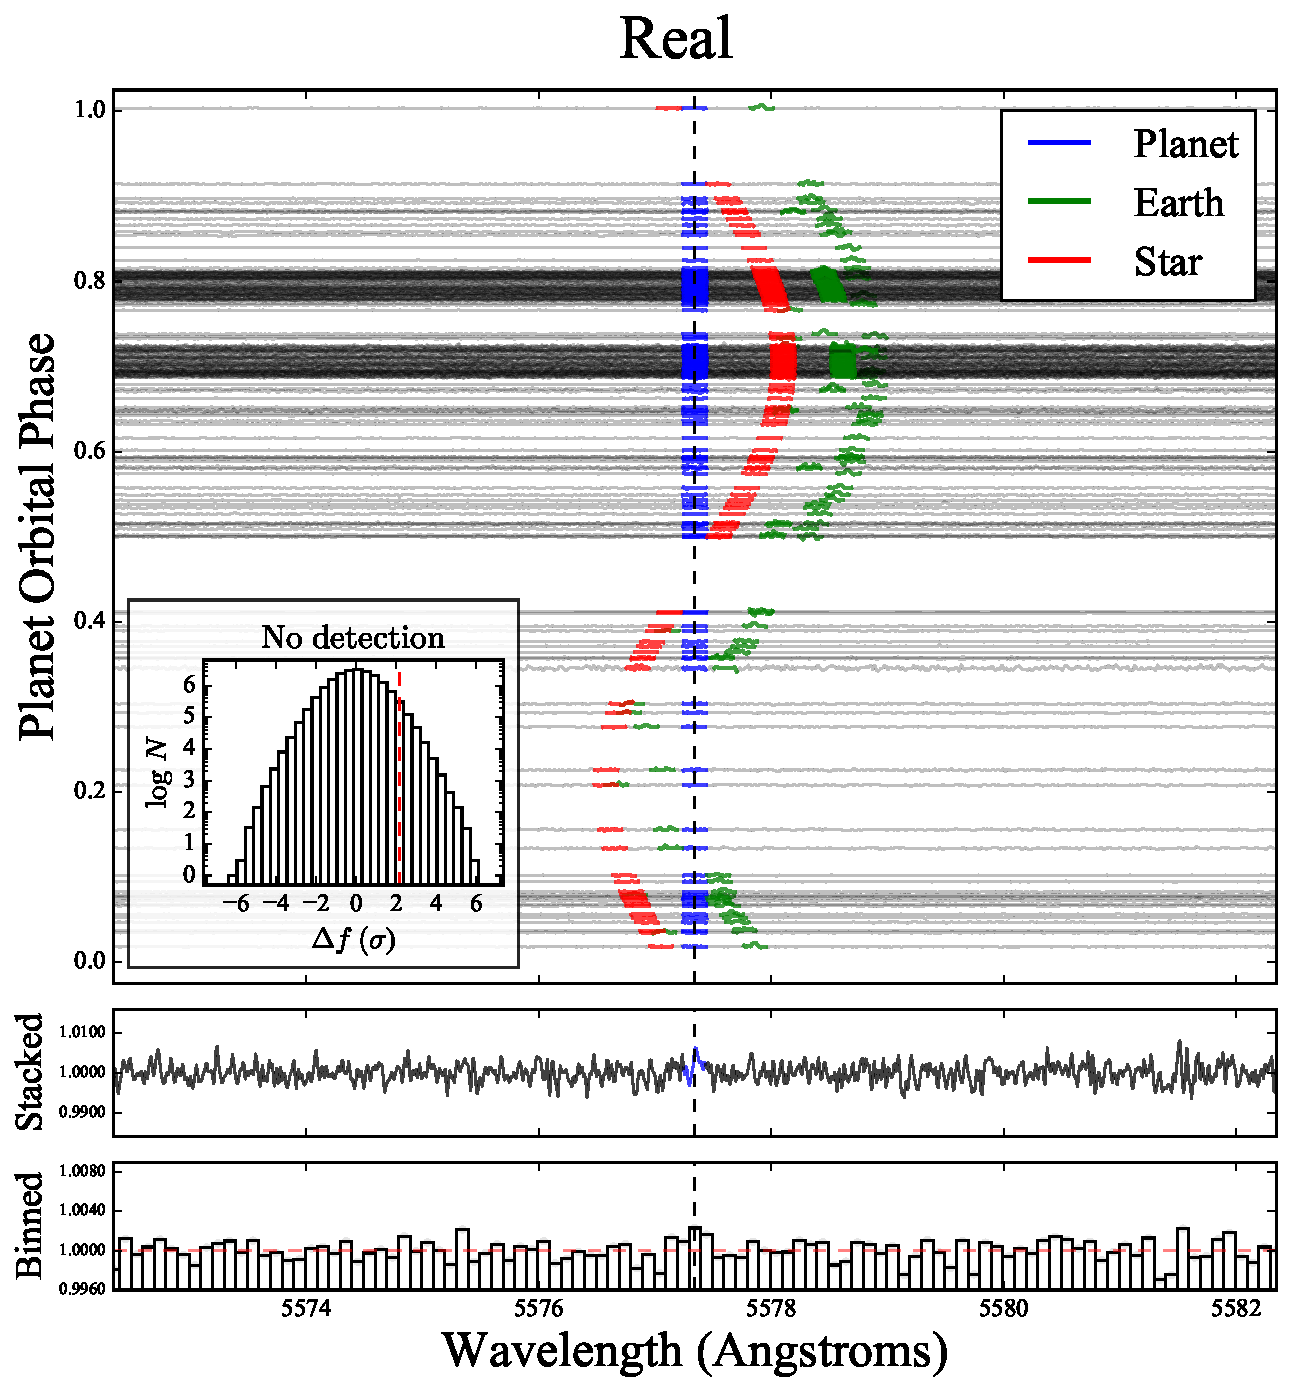
\includegraphics[width=0.47\textwidth]{real.pdf}}
\hspace{0.1in}
\subfigure{\label{fig:detection:b}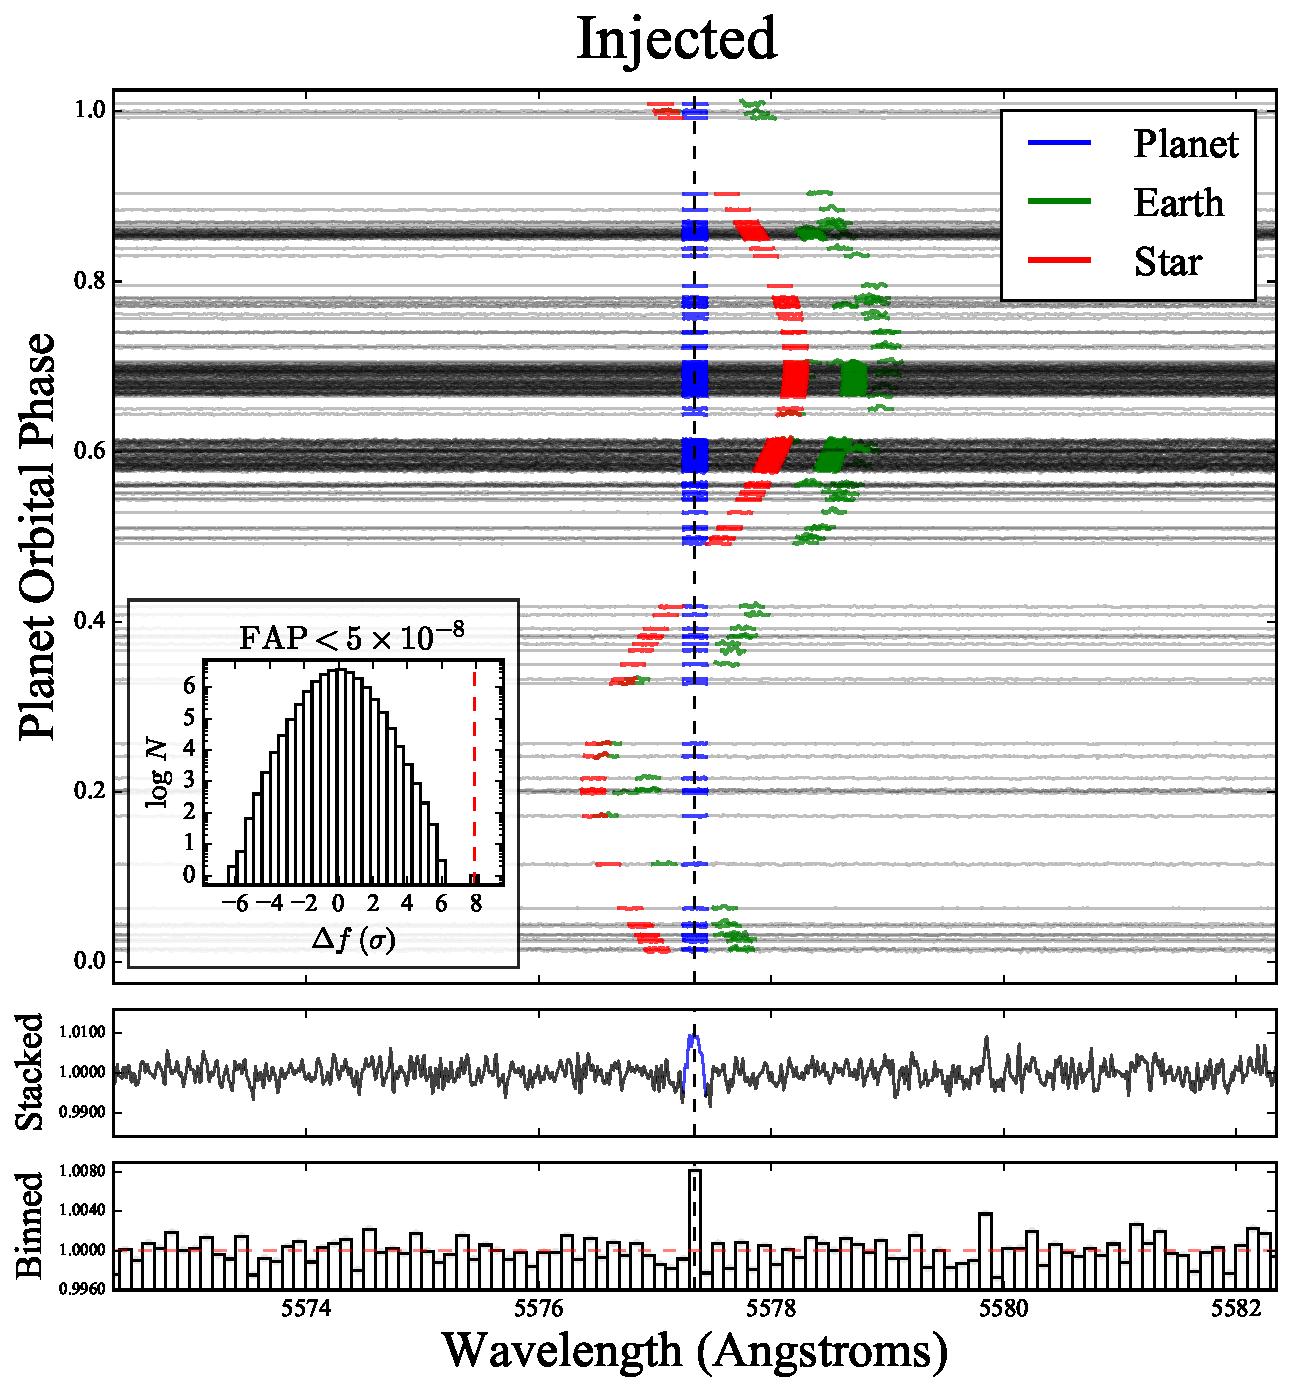
\includegraphics[width=0.47\textwidth]{strong.pdf}}
\caption{Analysis of the HARPS spectra of Proxima Centauri. After removing stellar and telluric lines, the individual spectra are Doppler-shifted into the frame of Proxima b and distributed vertically on the main subplots according to the planet's orbital phase. Blue regions indicate a 0.2\AA\ window centered on the 5577\AA\ oxygen feature in the planet frame. Red and green regions indicate the same window in the star and Earth frames, respectively; note the residual telluric airglow features in many of the spectra. The bottom subplots show the stacked spectrum in the planet frame and the stacked spectrum after downsampling to bins of size equal to the FWHM of the line. \emph{Left column}: Our search results, assuming an orbital inclination of $69^\circ$, which yields the strongest signal. The inset at the bottom left shows a histogram of the amplitude of the deviations from the median computed over a 250\AA\ window by randomly Doppler-shifting the spectra by small amounts and stacking them. The recovered signal is consistent with noise. \emph{Right column}: Results for an emission feature injected into the raw data with contrast $8\times 10^{-3}$. Our method recovers the signal in the stacked, binned spectrum at $8\sigma$.  From the histogram in the inset, we compute a false alarm probability (FAP) $\ll 5\times 10^{-8}$. The non-detection in the left panel therefore constrains the auroral power on Proxima b to be $\lesssim 4\times 10^{15}$ W, consistent with the calculations in \S\ref{sec:signal}.}
\label{fig:detection}
\end{figure*}

We find a peak at 5577\AA\ for an orbital inclination of $69^\circ$, but this ${\sim} 2.3 \sigma$ signal is entirely consistent with noise; see the left panel of Fig.~\ref{fig:detection}. In order to use this non-detection to constrain the auroral power of Proxima b, we performed injection/recovery tests to assess the efficiency of our retrieval method. We injected Gaussian OI emission features with FWHM = 0.1\AA\ and varying planet-star contrast into each of the raw spectra in the planet frame, and processed the spectra as explained above. Although we are able to detect the injected signal at $> 3\sigma$ down to a contrast ratio of $5\times 10^{-3}$, we note that a much larger detection threshold is necessary for a robust detection, particularly given the fact that we stacked the spectra in 3,500 different ways to search for a signal. We therefore estimate our false alarm probability (FAP) as a function of the amplitude of the recovered signal by randomly shifting, stacking, and binning the processed spectra $5,000$ times and computing a histogram of the deviations from the mean in each of the bins. We find that only one of ${\sim} 10^7$ bins had a signal $> 6\sigma$ from the mean. We therefore conservatively choose $8\sigma$ as the threshold for detection of OI emission from the planet, for which FAP $< 5\times 10^{-8}$ (though likely lower than this value by a few orders of magnitude). In the HARPS dataset, this corresponds to a contrast ratio of $8\times 10^{-3}$ (right panel of the figure). Based on Table~\ref{tab:OI_detect}, this constrains the auroral power of Proxima b to be $\lesssim 4\times 10^{15}$ W, consistent with the upper limits presented in \S\ref{sec:signal}.

We also performed similar searches for the red oxygen lines (6300 and 6364\AA) and the 3914\AA\ UV nitrogen line, which are prominent in Earth's aurora, but find no signal for any orbital configuration. Given the lower power in the red lines relative to the green line, and the low transmissivity of Earth's atmosphere and lower detector efficiencies in the UV, this non-detection is consistent with the non-detection of the 5577\AA\ feature.
  
\section{Discussion and Conclusions}
\label{sec:disc}

Given the RV estimate of Proxima b's mass of $m {\sin} i \approx 1.27\mathrm{M_\oplus}$, the planet is likely terrestrial \citep{Anglada-Escude2016}. However, due to the mass-inclination degeneracy, it is possible that Proxima b is more massive and on a close to face-on orbit, in which case it may be a mini-Neptune. In this case, its atmosphere may be dominated by H and He rather than by oxygen-bearing species. As we discussed in \S\ref{sec:signal}, a search for Lyman-Werner H$_2$ emission in the UV would be more appropriate in this case. Although broader than the lines we consider here, this emission is likely stronger (see \S\ref{sec:signal}), and is unlikely to be confused with stellar emission, given that it is molecular in origin. But perhaps more importantly, a robust \textit{non}-detection of this and other H/He features could rule out a large gaseous envelope and confirm the terrestrial nature of the planet. That said, we are currently unable to efficiently probe near-face-on orbits due to the much smaller Doppler shift of the planetary lines. Observations made exclusively at quadrature, when the planet RV is highest, may help with this in the future.

In the more likely case that Proxima b is terrestrial, our HARPS search constrains its auroral power to be $< 4\times 10^{15}$ W. This is consistent with the calculations in \S\ref{sec:signal}, which suggest the auroral power on Proxima b is likely on the order of $10^{12}$ W, or $\sim 100\times$ that of the Earth during steady-state solar wind conditions. Those calculations, however, ignore transient increases in stellar magnetic activity, which can enhance the auroral signal, and the diffuse airglow emission of the planet. As discussed in \S\ref{sec:signal}, transient magnetospheric activity could result in auroral power on the order of $10^{13}$ W. Future spectroscopic observations of Proxima Centauri may thus wish to observe during periods of vigorous magnetospheric activity.

Even if Proxima b is terrestrial, an auroral signal is not guaranteed to be present. The existence of an atmosphere is still an open question, owing to vigorous past hydrodynamic escape \citep{LugerBarnes2015, Barnes2016}, persistent stellar activity \citep{Davenport2016} and an unconstrained planetary magnetic field. Even if an oxygen-rich atmosphere is present, nitrogen may need to be present to enhance the auroral signal. On Earth, ${\sim}40\%$ of the OI green line emission results from collisions with excited N$_2^+$ \citep{Strickland2000}. It is unclear whether or not other molecular species could play a similar role if N$_2$ is not the bulk atmospheric constituent. However, the detection of the 3914\AA\ N$_2^+$ line could be a good diagnostic in the UV, where the star is even fainter. If we assume that the power of the 3914\AA\ nitrogen line is comparable to that of the OI line (which is typical for higher energy magnetospheric particle populations), then the planet-star contrast in the N$_2^+$ line is an order of magnitude greater than at 5577\AA. Since the strength of the N$_2^+$ line scales with magnetospheric parameters, stellar activity could cause strong transient features in the UV, which may be observable. Note, however, that limitations in UV detector efficiencies may complicate the detection of nitrogen and other UV aurorae.

A detection of an exo-aurora using the methods presented in \S\ref{sec:search} would place strong constraints on the eccentricity and break the $m {\sin} i$ degeneracy, leading to greater confidence in the terrestrial nature of Proxima b. Our non-detection places no such constraints, but our predicted telescope integration times of order 100 hours outline a path towards detecting auroral emission with reasonable upgrades to current and future facilities. We encourage further research into the use of high resolution spectroscopy with coronagraphic starlight suppression, particularly using low noise detectors that will allow substantial spectral downbinning with minimal added noise. Additionally, the development of effective optical AO and high contrast imaging systems is crucial for future observations aimed at optical auroral detection. 

Our integration times using LUVOIR and HabEx suggest that they can be excellent observatories for the observation of aurora.  However, such measurements would required a high resolution mode similar to the SPHERE and ESPRESSO coupling \citep{Lovis2016}.  Furthermore, since read noise and dark current dominate the coronagraph noise budget, the development of low-noise detectors, e.g. MKIDS \citep{Mazin2012,Mazin2015}, would significantly help the detection sensitivity and would allow such high-resolution spectroscopy to be downbinned to the lower resolution typically considered for direct exoplanet spectroscopy.

The methods of exo-auroral detection discussed here are not limited to Proxima b, but may be applicable to any exoplanet orbiting a nearby late-type star or brown dwarf.  For example, the recently discovered TRAPPIST-1 system \citep{Gillon2016} consists of three planets orbiting an active late M8 ultracool dwarf only 12 pc away; one planet in the system, TRAPPIST-1d, potentially lies in the habitable zone. Since TRAPPIST-1 is a later type star than Proxima Centauri, it is likely more active \citep[e.g.,][]{West2008} and hence could generate larger particle fluxes and a stronger interplanetary magnetic field than Proxima Centauri, leading to more powerful aurorae on its planets. Additionally, TRAPPIST-1 is roughly $5\times$ dimmer than Proxima Centauri at the OI $5577$\AA\ line, resulting in far more favorable contrast ratios. However, due to its distance, auroral emission from this system will be $\sim 100\times$ dimmer than that from Proxima Centauri, likely making its detection infeasible. For coronagraphic observations, the distance to the TRAPPIST system would require an inner working angle smaller than the diffraction limit to extend as long as 5577\AA\ for all known TRAPPIST-1 planets observed with a 10m class telescope, further complicating the observation.

Another planet to consider is GJ1132b, which orbits a M3.5 star 12 pc away \citep{Berta2015}. Since it receives $\sim 19\times$ the Earth's flux and may have an O$_2$ rich atmosphere \citep{Schaefer2016}, it could display strong auroral emission. However, as with the TRAPPIST-1 system, its distance makes auroral characterization difficult. Moreover, the earlier type host emits a larger fraction of its light in the optical, resulting in a poorer auroral contrast ratio.

Finally, exoplanets orbiting nearby brown dwarfs may be prime targets for exo-auroral searches. Although no short-period exoplanets are currently known to orbit nearby brown dwarfs \citep{He2016}, the methods described in this paper may be used as means of exoplanet detection. Since the stack-and-search method described in \S\ref{sec:search} does not require previous RV observations of a system, a long baseline of spectroscopic observations of nearby M dwarfs and brown dwarfs could be used to search for Doppler-shifted 5577\AA\ OI emission. Our method is particularly sensitive to short-period terrestrial planets, whose auroral power (if an atmosphere is present) is large and whose large RV will Doppler-shift the signal by one or more \AA. Future high-resolution spectroscopy observations of our nearest neighbors could thus reveal the presence of unknown terrestrial exoplanets, including ones in the habitable zone.

 %% Acknowledgements %%
\section{Acknowledgements}
\label{sec:ack}

We thank G. Anglada-Escude and the Pale Red Dot team for making their data publicly available. We thank Giada Arney for useful discussions. DPF is supported by an NSF IGERT DGE-1258485 fellowship. This work was supported by the NASA Astrobiology Institute’s Virtual Planetary Laboratory under Cooperative Agreement number NNA13AA93A.

%% Bibliograph %%
\bibliography{bib}

%% End Doc
\end{document}  
